% !TEX encoding = UTF-8 Unicode
\documentclass[a4paper]{article}

\usepackage{color}
\usepackage{url}
\usepackage[T2A]{fontenc} % enable Cyrillic fonts
\usepackage[utf8]{inputenc} % make weird characters work
\usepackage{graphicx}

\usepackage[english,serbian]{babel}
%\usepackage[english,serbianc]{babel} %ukljuciti babel sa ovim opcijama, umesto gornjim, ukoliko se koristi cirilica

\usepackage[unicode]{hyperref}
\hypersetup{colorlinks,citecolor=blue,filecolor=green,linkcolor=blue,urlcolor=blue}

\usepackage{listings}

%\newtheorem{primer}{Пример}[section] %ćirilični primer
\newtheorem{primer}{Primer}[section]

\definecolor{mygreen}{rgb}{0,0.6,0}
\definecolor{mygray}{rgb}{0.5,0.5,0.5}
\definecolor{mymauve}{rgb}{0.58,0,0.82}

\lstset{ 
  backgroundcolor=\color{white},   % choose the background color; you must add \usepackage{color} or \usepackage{xcolor}; should come as last argument
  basicstyle=\scriptsize\ttfamily,        % the size of the fonts that are used for the code
  breakatwhitespace=false,         % sets if automatic breaks should only happen at whitespace
  breaklines=true,                 % sets automatic line breaking
  captionpos=b,                    % sets the caption-position to bottom
  commentstyle=\color{mygreen},    % comment style
  deletekeywords={...},            % if you want to delete keywords from the given language
  escapeinside={\%*}{*)},          % if you want to add LaTeX within your code
  extendedchars=true,              % lets you use non-ASCII characters; for 8-bits encodings only, does not work with UTF-8
  firstnumber=1000,                % start line enumeration with line 1000
  frame=single,	                   % adds a frame around the code
  keepspaces=true,                 % keeps spaces in text, useful for keeping indentation of code (possibly needs columns=flexible)
  keywordstyle=\color{blue},       % keyword style
  language=Python,                 % the language of the code
  morekeywords={*,...},            % if you want to add more keywords to the set
  numbers=left,                    % where to put the line-numbers; possible values are (none, left, right)
  numbersep=5pt,                   % how far the line-numbers are from the code
  numberstyle=\tiny\color{mygray}, % the style that is used for the line-numbers
  rulecolor=\color{black},         % if not set, the frame-color may be changed on line-breaks within not-black text (e.g. comments (green here))
  showspaces=false,                % show spaces everywhere adding particular underscores; it overrides 'showstringspaces'
  showstringspaces=false,          % underline spaces within strings only
  showtabs=false,                  % show tabs within strings adding particular underscores
  stepnumber=2,                    % the step between two line-numbers. If it's 1, each line will be numbered
  stringstyle=\color{mymauve},     % string literal style
  tabsize=2,	                   % sets default tabsize to 2 spaces
  title=\lstname                   % show the filename of files included with \lstinputlisting; also try caption instead of title
}

\begin{document}

\title{Razvoj LSTM neuronske mreže i primena nad problemom sekvencijalnog učenja\\ \small{Seminarski rad u okviru kursa\\Računarska inteligencija\\ Matematički fakultet}}

\author{Nevena Soldat, Milena Kurtić\\ nevenasoldat@gmail.com, mimikurtic67@gmail.com}

%\date{9.~april 2015.}

\maketitle

\abstract{
U okviru ovog rada predstavljen je primer implementacije LSTM neuronske mreže u programskom jeziku Python, uz korišćenje biblioteka za rad kao što su pandas, numpy, keras i druge. Problem koji rešavamo jeste predviđanje broja obolelih osoba, kao i broja smrtnih slučajeva od virusa koji je zahvatio čitav svet. Videćemo koje su prednosti navedene vrste neuronskih mreža, kao i koja su njena ograničenja. Takođe ćemo se poslužiti jednom od dobro poznatih statističkih metoda koje rade sa ovom vrstom podataka i uporedićemo dobijene rezultate oba modela.
}

\tableofcontents

\newpage

\section{Uvod}
\label{sec:uvod}
Rekurentne neuronske mreže (eng. Recurrent Neural Networks - RNN) predstavljaju arhitekturu mreža specijalizovanu za obradu sekvencijalnih podataka, poput rečenica prirodnog jezika i vremenskih serija. One su konstruisane sa idejom da se modeluje zavisnost među instancama. Eksperimenti su pokazali da ih je veoma teško trenirati efikasno. Naime, prilikom ažuriranja težina, može doći do toga da njihova promena bude toliko mala da nema efekta (dovodi do problema nestajućih gradijenata), odnosno toliko velika da su promene prevelike (dovodi do problema eksplodirajućih gradijenata). Ovaj problem se prevazilazi upotrebom duge kratkoročne memorije (eng. long short term memory - LSTM), što je složena jedinica mreže sa specifičnom strukturom koja omogućava kontrolu čitanja i upisa u jedinicu. Upravo ova vrsta jedinice dovela je do ključnih uspeha rekurentnih neuronskih mreža, i predstavlja standardni izbor prilikom formulisanja modela rekurentne mreže \cite{matf}. 

\subsection{Primena na vremenske serije}
Predviđanje vremenskih serija se može opisati kao proces koji izvlači korisne informacije iz vrednosti koje su se realizovale u nekom prethodnom trenutku, i na osnovu njih predviđa buduće vrednosti. Nailazimo na veliku primenu ove tehnike u oblastima poput vremenske prognoze, planiranja transporta, odnosno regulisanja saobraćaja. Metode predviđanja koje su bazirane na neuronskim mrežama stiču veliku popularnost jer je dokazano da mogu biti podjednako dobre kao klasične statističke metode \cite{siami2018forecasting}. 
Analiza vremenskih serija i predviđanje su predmet intenzivnog proučavanja poslednjih 40 godina. Statistički model ARIMA (eng. Autoregressive Integrated Moving Average) je zbog svoje uspešnosti često korišćen za analizu procesa koji su vremenski zavisni. Međutim, glavno ograničenje ovog modela je to što ima tendenciju da teži ka srednjim vrednostima. 

\section{LSTM neuronske mreže}
Osnovna ideja LSTM-a je postojanje takozvane ćelije koja čuva skriveno stanje, uz kontrolu pisanja, čitanja i zaboravljanja, koja se vrši na osnovu naučenih pravila. Na slici \ref{fig:jedinica} prikazana je struktura LSTM jedinice, koja prikazuje ćeliju u centru i nekoliko kapija koje kontrolišu prethodno pomenute aspekte. Svaka od kapija ima strukturu kao jedinica standardne rekurentne mreže i na osnovu ulaza koje dobija i pridruženih im parametara odlučuje o tome da li i u kolikoj meri dozvoljava izvršavanje operacije koju kontroliše. Kapija koja kontroliše zaboravljanje odlučuje šta je bitno sačuvati iz prethodnog koraka. Ulazna kapija odlučuje koje informacije treba dodati iz trenutnog koraka. Izlazna kapija određuje sledeće skriveno stanje. Prednost LSTM jedinice je to što ćelija ne mora da prihvata ulazne signale, i stoga može dugo da čuva informaciju o dalekim delovima sekvence. 

\begin{figure}[htp]
    \centering
    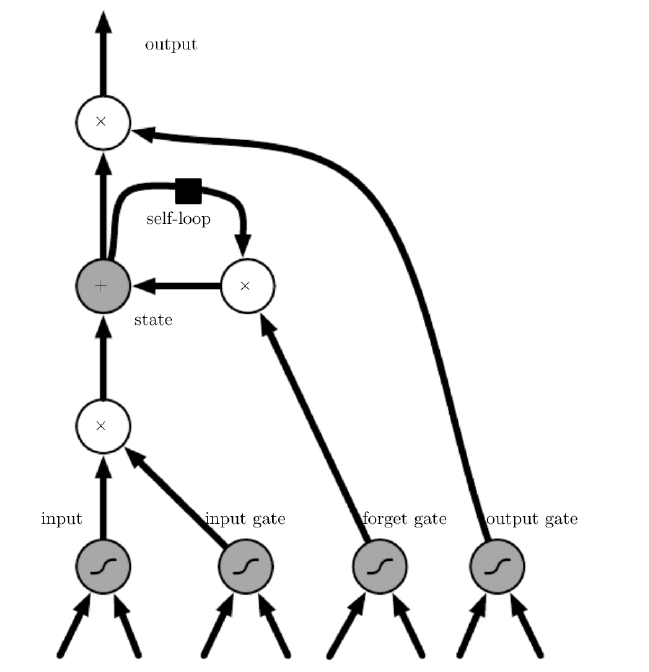
\includegraphics[scale=0.4]{lstm.png}
    \caption{Struktura LSTM jedinice}
    \label{fig:jedinica}
\end{figure}



\section{Opis problema}
Cilj ovog rada je demonstriranje upotrebe LSTM neuronske mreže na problem predviđanja vremenskih serija. Kako je predviđanje toka pandemije virusa u trenutku pisanja ovog rada jedna od najektuelnijih tema, podaci koje koristimo predstavljaju broj obolelih, kao i broj žrtava zaraze ovim virusom. Zadatak je predvideti kako će se ovi brojevi menjati kroz dane koji slede. Kako bismo pokazali uspešnost ove metode, uporedićemo je sa ranije pomenutom metodom ARIMA. 

\subsection{Opis baze podataka}
Za potrebe ovog projekta korišćena je baza podataka COVID19 Global Forecasting koja se u trenutku razvijanja ovog projekta svakodnevno ažurira (može se pronaći na sledećoj adresi: \url{https://www.kaggle.com/c/covid19-global-forecasting-week-3}). Baza sadrži podatke o broju osoba koje su potvrđeno zaražene virusom COVID-19, broj osoba koje su preminule, datume po danima počevši od 22.1.2020, kao i pokrajine i države na koje se date brojke odnose. Podaci su smešteni u fajl pod nazivom train.csv. 

\section{Rešenje problema}
Problem predviđanja toka pandemije virusa rešavamo pomoću LSTM neuronske mreže. Program se sastoji iz sledećih delova:
\begin{itemize}
    \item \textbf{Preprocesiranje}
    \item \textbf{Konfiguracija modela}
    \item \textbf{Testiranje modela}
\end{itemize}


\subsection{Preprocesiranje}
Kako bismo primenili LSTM neuronske mreže moramo da sredimo podatke koje imamo. To, u ovom slučaju, podrazumeva popunjavanje nedostajućih vrednost kao i normalizaciju podataka.


Nedostajuće vrednosti imamo u koloni Province\_State. Te vrednosti popunjavamo sa vrednostima iz kolone Country\_Region, što je prikazano na slici \ref{fig:Pretprocesiranje1}.  
\begin{figure}[htp]
    \centering
    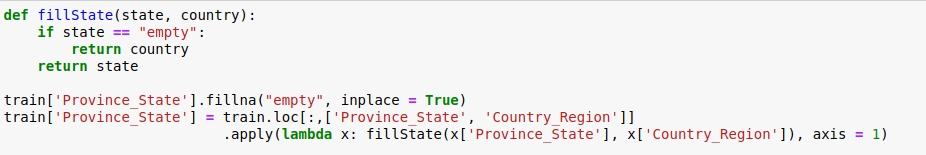
\includegraphics[scale=0.5]{preprocesiranje1.png}
    \caption{Popunjavanje nedostajućih vrednosti}
    \label{fig:Pretprocesiranje1}
\end{figure}

Kada mreža koristi podatke koji su u velikom rasponu vrednosti, za velike ulaze može doći do velikog usporavanja učenja kao i konvergencije, stoga je potrebno skalirati date podatke. Postoje dva nacina za skaliranje vrednosti:

\begin{itemize}
    \item \textbf{Normalizacija}: Ponovno skaliranje vrednosti podataka tako da su svi u opsegu od 0 do 1.
    \item \textbf{Standardizacija}: Reskaliranje vrednosti podataka tako da je srednja vrednost 0 a standardna devijacija 1.
\end{itemize}

Za potrebe ovog projekta korišćena je normalizacija (Standardizaciju ima smisla koristiti kada bi imali Gausovu raspodelu). Normalizaciju datog skupa podataka vršimo pomoću biblioteke scikit-learn i objekta MinMaxScaler.\ref{fig:Pretprocesiranje2}

\begin{figure}[htp]
    \centering
    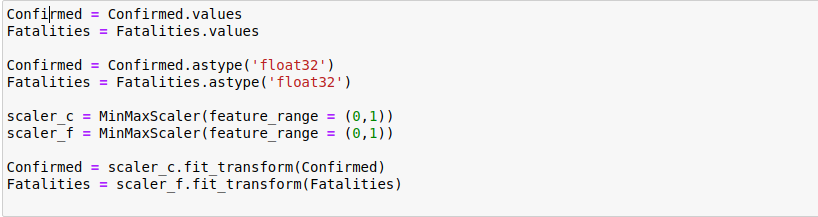
\includegraphics[scale=0.5]{preprocesiranje2.png}
    \caption{Normalizacija podataka}
    \label{fig:Pretprocesiranje2}
\end{figure}

Kako bi podaci bili u odgovarajućem obliku, vršimo transformaciju na sledeći način. Odvajamo podatke za broj obolelih od podataka za broj smrtnih slučajeva. U oba slučaja kolona za datum postaje indeks, dok različite države smeštamo po kolonama. Tako imamo za svaku državu broj slučajeva uređene po danima. Početni datum je 22.01.2020, a broj država u ovom trenutku je 184. Model koji gradimo radi sa brojem instanci koji je jednak broju dana za koje imamo podatke, i paralelno vrši predviđanje za sve države. 

\subsection{Konfiguracija modela}
Kako podaci koje imamo predstavljaju vremenske serije, sami moramo formirati ulaz, odnosno izlaz iz mreže. Ulaz je predstavljen podacima za tri dana uzastopno, dok je izlaz broj za četvrti dan. 
Funkcija split\_sequences (sequences, n\_steps\_in, n\_steps\_out) obavlja taj zadatak. LSTM sloj zahteva da ulazni podaci budu u sledećem obliku - (n\_samples, n\_steps, n\_features)\footnote{n\_samples predstavlja broj uzoraka, n\_steps broj koraka, a n\_features broj izlaza}, odnosno da imaju tri dimenzije. Prethodno opisana funkcija nam baš to omogućava. 

Sledeći korak je podela podataka na trening i test skup. Kako funkcija train\_test\_split podelu vrši na nasumičan način, mi je ne možemo koristiti. Vremenske serije zahtevaju da ostane održano uređenje podataka. Podelu radimo ručno, 80\% podataka je odvojeno za trening, a 20\% za test. 

\subsubsection{Model za broj potvrđenih slučajeva}

\subsubsection{Model za broj smrtnih slučajeva}

\subsection{Testiranje modela}


\section{Zaključak}
\label{sec:zakljucak}


\addcontentsline{toc}{section}{Literatura}
\appendix
\bibliography{bibliography.bib} 
\bibliographystyle{plain}

\appendix
\section{Dodatak}

\end{document}

